\documentclass{article}
\usepackage[margin=1in]{geometry}
\usepackage{amsmath,amsthm,amssymb}
\usepackage{bbm,enumerate,mathtools}
\usepackage{tikz,pgfplots}
\usepackage{chessboard}
\usepackage[hidelinks]{hyperref}
\usepackage{multicol} % Problem 35
\usepackage{xstring} % Difficulty command
\usetikzlibrary{shapes.geometric}

\newenvironment{question}{\begin{trivlist}\item[\textbf{Question.}]}{\end{trivlist}}
\newenvironment{note}{\begin{trivlist}\item[\textbf{Note.}]}{\end{trivlist}}
\newenvironment{references}{\begin{trivlist}\item[\textbf{References.}]}{\end{trivlist}}
\newenvironment{related}{\begin{trivlist}\item[\textbf{Related.}]\end{trivlist}\begin{enumerate}}{\end{enumerate}}

\newcommand\score[1]{
\pgfmathsetmacro\pgfxa{#1+1}
\tikzstyle{scorestars}=[
  star,
  star points=5,
  star point ratio=2.25,
  draw,
  inner sep=3pt,
  anchor=outer point 5
]
  \begin{tikzpicture}[baseline]
    \draw[opacity=0] (0,-0.5) rectangle (0,0.2); % Workaround for whitespace at the bottom.
    \foreach \i in {1,...,4} {
      \pgfmathparse{(\i<=#1?"yellow":"gray")}
      \edef\starcolor{\pgfmathresult}
      \draw (\i*4.5ex,0) node[name=star\i,scorestars,fill=\starcolor]  {};
    }
  \end{tikzpicture}
}

\newcommand{\difficulty}[1]{%
  \IfEqCase{#1}{%
      {1}{
        
\begin{tikzpicture}[scale=0.7, baseline=0.9mm]%
          \definecolor{slopegreen}{rgb}{0.0, 0.5, 0.0}%
          \fill[slopegreen] (0.5,0.5) circle (0.5);%
        \end{tikzpicture}%
      }%
      {2}{
        
\begin{tikzpicture}[scale=0.7, baseline=0.9mm]%
          \definecolor{slopeblue}{rgb}{0.0, 0.44, 1.00}
          \fill[slopeblue] (0,0) rectangle (1,1);%
        \end{tikzpicture}%
      }%
      {3}{
\begin{tikzpicture}[scale=0.7, baseline=0.9mm]\fill (0,0.5)--(0.5, 0)--(1,0.5)--(0.5,1)--cycle; \end{tikzpicture}}%
      {4}{
\begin{tikzpicture}[scale=0.7, baseline=0.9mm]\fill (0.25,0)--(0,0.5)--(0.25,1)--(0.5,0.5)--cycle; \fill (0.75,0)--(0.5,0.5)--(0.75,1)--(1,0.5)--cycle;\end{tikzpicture}}%
      % you can add more cases here as desired
  }[\PackageError{difficulty}{Undefined difficulty level: #1}{}]%
}%
\newcommand{\rating}[2]{\difficulty{#1}\\\score{#2}\\}


\begin{document}
  Conside equivalence classes of polygonal chains on $n$ segments where
  \begin{enumerate}[(1)]
    \item Edges can cross, but no segment can have a vertex on another segment's
      edge.
    \item Two chains are equivalent if one can move to the other without an edge
    crossing over a vertex, or a crossing being otherwise changed.
  \end{enumerate}
  \begin{figure}[ht!]
    \centering
    
\begin{tikzpicture}
      \draw[line width=0.1cm] (0,0)--(0,1)--(1,1)--(1,0)--(0,0);
    \end{tikzpicture}\hspace{1cm}
    
\begin{tikzpicture}
      \draw[line width=0.1cm] (0,0)--(0,1)--(1,0)--(1,1)--(2,0);
    \end{tikzpicture}\hspace{1cm}
    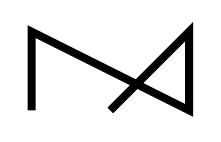
\begin{tikzpicture}
      \draw[line width=0.1cm] (0,0)--(0,1)--(2,0)--(2,1)--(1,0);
    \end{tikzpicture}\hspace{1cm}
    
\begin{tikzpicture}
      \draw[line width=0.1cm] (0,0)--(2,1)--(2,0)--(1,1)--(1,0);
    \end{tikzpicture}\hspace{1cm}
    
\begin{tikzpicture}
      \draw[line width=0.1cm] (0,0)--(0,1)--(1,1)--(1,0)--(0,1);
    \end{tikzpicture}\\~\\
    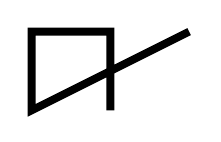
\begin{tikzpicture}
      \draw[line width=0.1cm] (2,1)--(0,0)--(0,1)--(1,1)--(1,0);
    \end{tikzpicture}\hspace{1cm}
    
\begin{tikzpicture}
      \draw[line width=0.1cm] (0, 0)--(1,1)--(1,0)--(0,0)--(2,1);
    \end{tikzpicture}\hspace{1cm}
    
\begin{tikzpicture}
      \draw[line width=0.1cm] (0, 0)--(1,1)--(0,1)--(1,0)--(0,0);
    \end{tikzpicture}\hspace{1cm}
    
\begin{tikzpicture}
      \draw[line width=0.1cm] (0, 0)--(2,1)--(1,0)--(0,1)--(2,0);
    \end{tikzpicture}\hspace{1cm}
    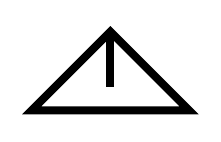
\begin{tikzpicture}
      \draw[line width=0.1cm] (0, 0)--(2,0)--(1,1)--cycle;
      \draw[line width=0.1cm] (1,1)--(1,0.3);
    \end{tikzpicture}
    \caption{
      Examples of all known classes of polygonal chains of length $4$.
    }
  \end{figure}
  \begin{question}
    How many classes of polygonal chains exist on $n$ segments?
  \end{question}

  \begin{related}
    \item What if all segments are of unit length, so the final example is not
      allowed?
    \item What if The fifth and seventh example are considered the same because
      they are isomorphic as graphs? (Even if vertices are added at each
      intersection)
  \end{related}
  \begin{references}
    \item Problem 61.
  \end{references}
\end{document}
